\subsection{Algoritmo Genético}
En terminos generales, un algoritmo genético se compone de 8 pasos:

\begin{enumerate}
	\item \textbf{Generar población inicial.} Se debe elegir de forma aleatoria $n$ posibles soluciones dentro del dominio de nuestro problema.
	\item \textbf{Codificar dominio.} Una vez seleccionadas las muestras, se deberá realizar un proceso de codificación, donde se buscará expresar a las posibles soluciones en términos de genes, individuos y población.
	\item \textbf{Evaluar aptitud.} Teniendo una población, se deberá evaluar la aptitud de estos mediante la definición de una función de aptitud. Esta función suele ser inversa a las funciones de costo.
	\item \textbf{Ordenar individuos.} La mayoría de los algoritmos genéticos suele seleccionar a las individuos más aptos, por lo que se recomienda ordenar de forma descendente a la población.
	\item \textbf{Seleccionar parejas.} Es un proceso en el que se forman parejas, las cuales en pasos posteriores se someterán a proceso de reproducción en los que se buscará mejorar los resultados.
	\item \textbf{Reproducción de individuos.} Habiendo seleccionado a los individuos que se reproducirán, se deberá definir un método mediante el cual se mezcle la información de estos.
	\item \textbf{Mutación.} En la naturaleza suele ocurrir en una proporción muy pequeña procesos de mutación, estos procesos consisten en proveer a los individuos hijos de características que no poseen los padres, lo cuál en algunas ocasiones puede generar una mejora en su aptitud.
	\item \textbf{Evaluar nueva generación.} Una vez que se ha realizado el proceso de cruza, se deberá evaluar que tan buenos son los individuos resultantes de la reproducción, esto será útil para en procesos posteriores determinar cuales serán los individuos que prevalezcan.
\end{enumerate}

\subsection{Mecanismos de selección}
Los mecanismos de selección permiten determinar de forma metódica cuáles serán los individuos que realizarán su reproducción.

\subsubsection{Selección poligámica aleatoria}
En la selección poligámica aleatoria se forma parejas de forma aleatoria, sin importar si algún individuo es emparejado más de 1 vez. Una desventaja de este método es que existe la posibilidad de no seleccionar a un individuo, lo cuál podría ocasionar que no se explore completamente el espacio de búsqueda. En la Figura \ref{fig: selection_poli} podemos observar una representación gráfica de este mecanismo de selección.

\begin{figure}[htbp]
	\centering
	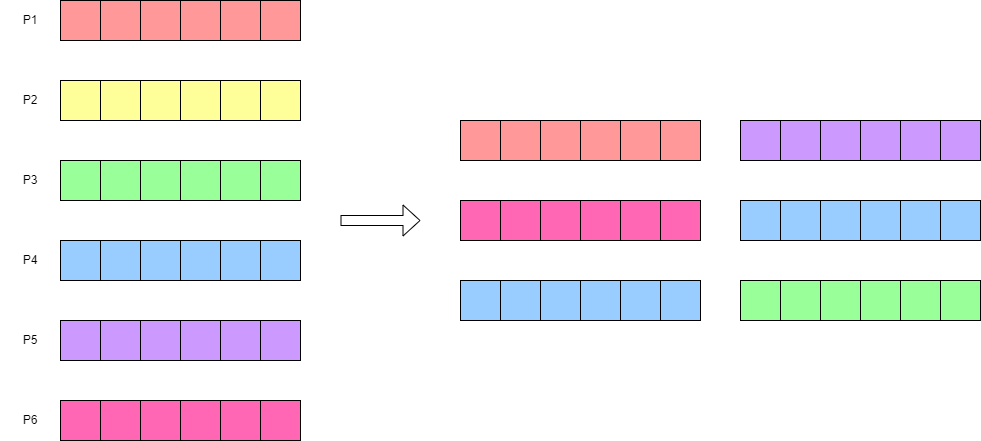
\includegraphics[width=0.8\textwidth]{random_poligamica}
	\caption{Mecanismo de selección poligámica aleatoria.}
	\label{fig: selection_poli}
\end{figure}

\subsubsection{Selección monogámica aleatoria}
Es un mecanismo similar a la selección monogámica aleatoria, con la peculiaridad de que una vez que un individuo a sido seleccionado, no se puede volver a seleccionar en esa generación. Este algoritmo garantiza que todos los individuos se reproduzcan, sin embargo, esto podría traer el problema de que prevalezcan individuos no aptos. La Figura \ref{fig: selection_mono} muestra una representación gráfica de este proceso.

\begin{figure}[htbp]
	\centering
	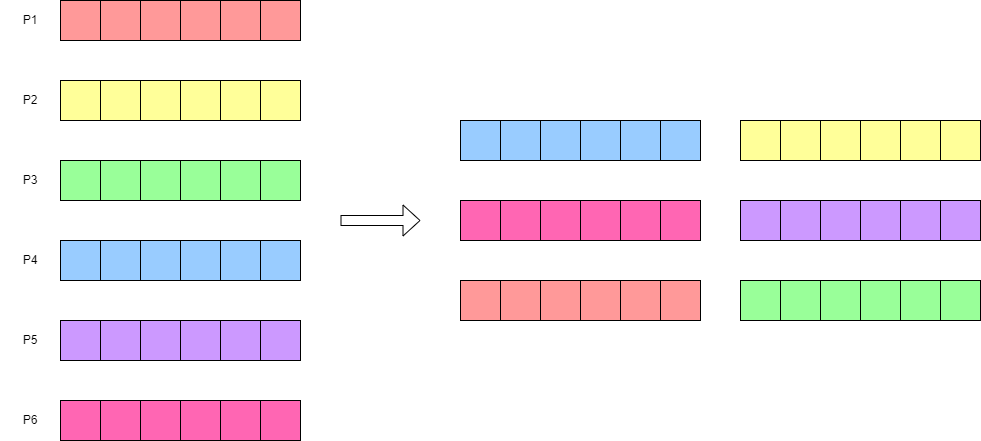
\includegraphics[width=0.8\textwidth]{random_monogamica}
	\caption{Mecanismo de selección monogámica aleatoria.}
	\label{fig: selection_mono}
\end{figure}

\FloatBarrier
\subsection{Mecanismos de reproducción}
Los mecanismos de reproducción establecen las reglas mediante las cuales los individuos mezclarán sus rasgos genéticos.

\subsubsection{Cruza de un punto}
En la cruza de un punto se define un punto por el que los individuos será dividido, usualmente se escoge la mitad de estos. Una vez que se han generado los cortes, se procede a realizar una combinación cruzada de estos. La Figura \ref{fig: cross_one} muestra este proceso de forma gráfica.

\begin{figure}[htbp]
	\centering
	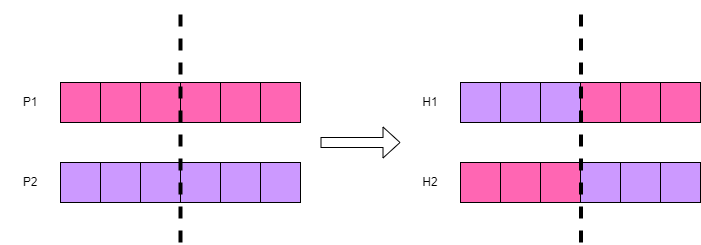
\includegraphics[width=0.8\textwidth]{crossover_one}
	\caption{Mecanismo de cruza de un punto.}
	\label{fig: cross_one}
\end{figure}

\subsubsection{Cruza de dos puntos}
Un proceo de cruza similar a la cruza de un punto, sin embargo, en este caso de definen dos puntos de corte y se realiza una combinación en forma de V entre los individuos. En la Figura \ref{fig: cross_two} se puede observar este proceso.

\begin{figure}[htbp]
	\centering
	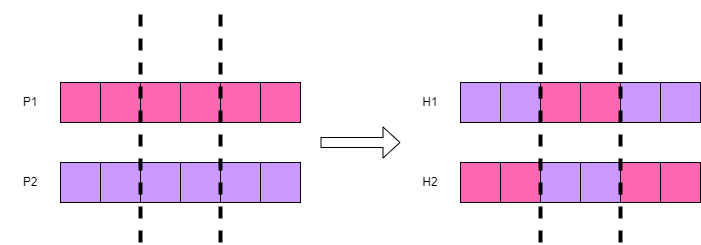
\includegraphics[width=0.8\textwidth]{crossover_two}
	\caption{Mecanismo de cruza de dos puntos.}
	\label{fig: cross_two}
\end{figure}

\subsection{Criterios elitistas}
La base de los algoritmos genéticos es la idea de que los individuos más aptos serán los que logren reproducirse y pasar su información genética a la siguiente generación, es por ello que los criterios elitistas buscan realizar un proceso de \textit{depuración} de los individuos, permitiendo que solamente prevalezcan los individuos más aptos.

\subsubsection{Competencia genética}
En este proceso se toma a todos los padres y a todos los hijos, se ordenan de mayor a menor aptitud, y solamente se permitirá que pasen a la siguiente generación aquellos que presentan mejor aptitud, sin importar sin son padres o hijos.